\documentclass{joel_cv}
\usepackage[colorlinks,linkcolor=red]{hyperref}
\usepackage{enumitem}
\usepackage{graphicx} 

\begin{document}
\pagestyle{empty}

% Name, phone, email, address
\begin{cvHeader} 
	\printName{Wen-tao Zhang (Toby)}
	\printPhone{(+86)156-006-04767}
	\printEmail{zwt@pku.edu.cn}
	%\printWebsite{http://nsknojj.github.io}
	%\printaddress{R505, CSIE Bldg., No. 1, Sec. 4, Roosevelt Rd., Taipei, Taiwan}
\end{cvHeader}

%
% Education
%

\sectionTitle{Education}
\begin{sectionContentSimple}{Peking University}{Sep. 2013 - Present}
	\item B.S. in Computer Science
	\begin{itemize}
		\item Overall GPA: 3.52/4.0 \quad Major GPA: 3.62/4.0
	\end{itemize}
	\item National Engineering Laboratory for Video Technology (NELVT), Video Coding Technology Lab
	\item Advisor: Siwei Ma
\end{sectionContentSimple}

%
% Experience
%

\sectionTitle{Experience}

\begin{sectionContentNormal}{Students' Association of College of EECS, Peking Univ.}{Sept. 2013 - June 2014}{Member of Acadamic Dept.}
	\item Organized several lectures about overseas studying and postgraduate recommendation
\end{sectionContentNormal}

\begin{sectionContentNormal}{Video Coding Technology Lab, Peking Univ.}{Apr. 2015 - Present}{Intern}
	\item Did research on High Efficiency Video Coding
\end{sectionContentNormal}

\begin{sectionContentNormal}{Zhang Research Group, Computer Systems Lab, Cornell Univ.}{July 2016 - Sept. 2016}{Intern}
	\item Did research project about Binarized Neural Network (BNN) Acceleration
\end{sectionContentNormal}


%
% Awards
%

\sectionTitle{Awards, Grants \& Honors}
\begin{description}{}
	\item{\ \ } International Olympiad in Informatics (IOI) 2013 China Team Selection Competition Ninth Place
	\item{\ \ } The ACM-ICPC Asia Regional Contest Chengdu Site 2013 Silver Medal (Twenty-third Place)
	\item{\ \ } Merit Student of Peking University, 2013 - 2014 Acadamic Year
	\item{\ \ } Tung OOCL Scholarship, 2013 - 2014 Acadamic Year
	\item{\ \ } The ACM-ICPC Asia Regional Contest Mudanjiang Site 2014 Gold Medal (Tenth Place)
\end{description}


%
% Projects
%

\sectionTitle{Projects}

\begin{sectionContentSimple}{Image Segmentation}{Jun. 2015}
\item A naive implementation based on Graph-Cut algorithm
\item \url{https://github.com/nsknojj/graph-cut-based-on-maxflow}
\end{sectionContentSimple}

\begin{sectionContentSimple}{Log File System}{Jan. 2016}
\item Designed a client caching mechanism for Hadoop Distributed File System (HDFS)
\item \url{https://github.com/nsknojj/LogFileSystem}
\end{sectionContentSimple}

\begin{sectionContentSimple}{Pedestrian and Car Detection on Dataset PKUSVD}{Nov. 2015 - Dec. 2015}
\item Neural network was based on Fast-RCNN, Proposal algorithm: ACF \& EdgeBox
\item \url{https://github.com/nsknojj/fast-rcnn-final}
\end{sectionContentSimple}

\begin{sectionContentSimple}{Birdway}{Oct. 2015 - Dec. 2015}
\item A collaborative editing plugin for Atom
\item \url{https://github.com/yangzhixuan/birdway} \quad \url{https://github.com/nsknojj/Birdway-Server}
\end{sectionContentSimple}

\begin{sectionContentSimple}{Video coding based on object features}{June 2015 - May 2016}
\item Built an application that can search for a similar frame in a video using extracted features
\end{sectionContentSimple}

\begin{sectionContentSimple}{Big File Upload plugin on Jupyter Notebook}{April 2016 - June 2016}
\item Add a plugin to upload big file on Jupyter Notebook
\item \url{https://github.com/nsknojj/notebook/tree/upload}
\end{sectionContentSimple}

\begin{sectionContentSimple}{Binarized Neural Network (BNN) acceleration project}{July 2016 - Sept. 2016}
\item Test the baseline of BNN, and implemented BNN with Halide, a language for parallelization and optimization
\item \url{https://github.com/nsknojj/bnn-halide} (private)
\end{sectionContentSimple}


%
%Technical Strengths
%

\sectionTitle{Strengths}
\begin{description}{}
	\item{\ \ } Computer Languages: C++, Python, JAVA, Shell Script
	\item{\ \ } Hobbies and Interests: table tennis, billiards, music, movie
\end{description}

%
% Publications
%

\sectionTitle{Publications}
%\begin{sectionItemize}{$\cdot$}
%\item \underline{Ting-Hsuan Chao}, Yen-Liang Lin, Yin-Hsi Kuo and Winston H. Hsu, "Scalable Object Detection by Filter Compression with Regularized Sparse Coding," Proceedings of the IEEE Conference on Computer Vision and Pattern Recognition, 2015. (Full paper)
%	\item Yu-Hsiu Chen, \underline{Ting-Hsuan Chao},  Yen-Liang Lin and Winston H. Hsu, "Filter-Invariant Image Classification on Social Media Photos," ACM Multimedia, 2015. (Short paper)
%	\item Wen-Yu Lee, Yin-Hsi Kuo, Peng-Ju Hsieh, Wen-Feng Cheng, \underline{Ting-Hsuan Chao}, Hui-Lan Hsieh, Chieh-En Tsai, Hsiao-Ching Chang, Jia-Shin Lan, Winston Hsu, "Unsupervised Latent Sub-events Discovery based on Multi-content and Human Activities Analysis for Diverse Event Summarization,"  ACM Multimedia, 2015. (Grand Challenge)
%\end{sectionItemize}

% For aesthetic
%\pagebreak


\sectionTitle{A Photo Taken at Brooklyn Bridge}
\centering 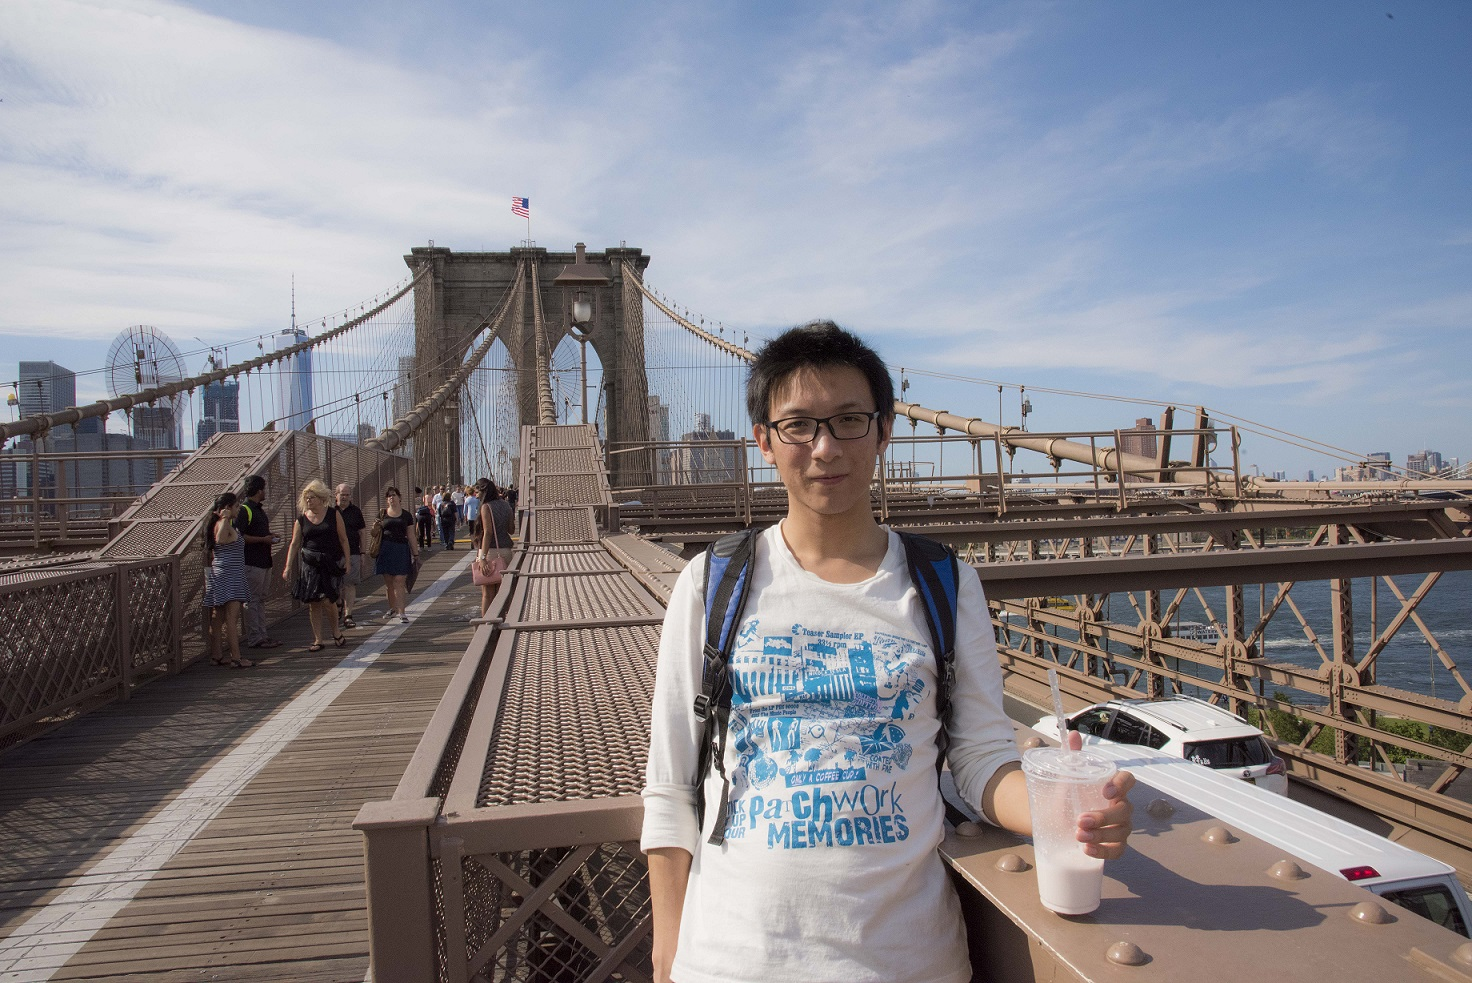
\includegraphics[height=4in]{brooklyn.jpg}

\end{document}

